


In lab3 we wrote the controller for the processor. We began by sketching a mealy
type final state machine using figure \ref{lab3_1:FSM} provided in the processor pdf file. This
could later be used in the vhdl code to determine the next state of the
processor by defining a process that depends on the current state and the opcode. 
Later, the output signals were defined by a process depending on current state,
opcode and the eq and neq flags. We begin this process by setting all the
outputs to zero and then we build all of the possible cases in a case statement
matching the opcodes to later set the outputs depending on current state. This
was probably the hardest part of the lab to debug the cases that did not give
the correct output. However, we found it very useful to carefully observe the
control signals per instruction in table 3 of the processor pdf while debugging
to correct the outputs. 

\begin{figure}[h]
    \caption{Mealy FSM of lab3.}
    \label{lab3_1:FSM}
    \centering
    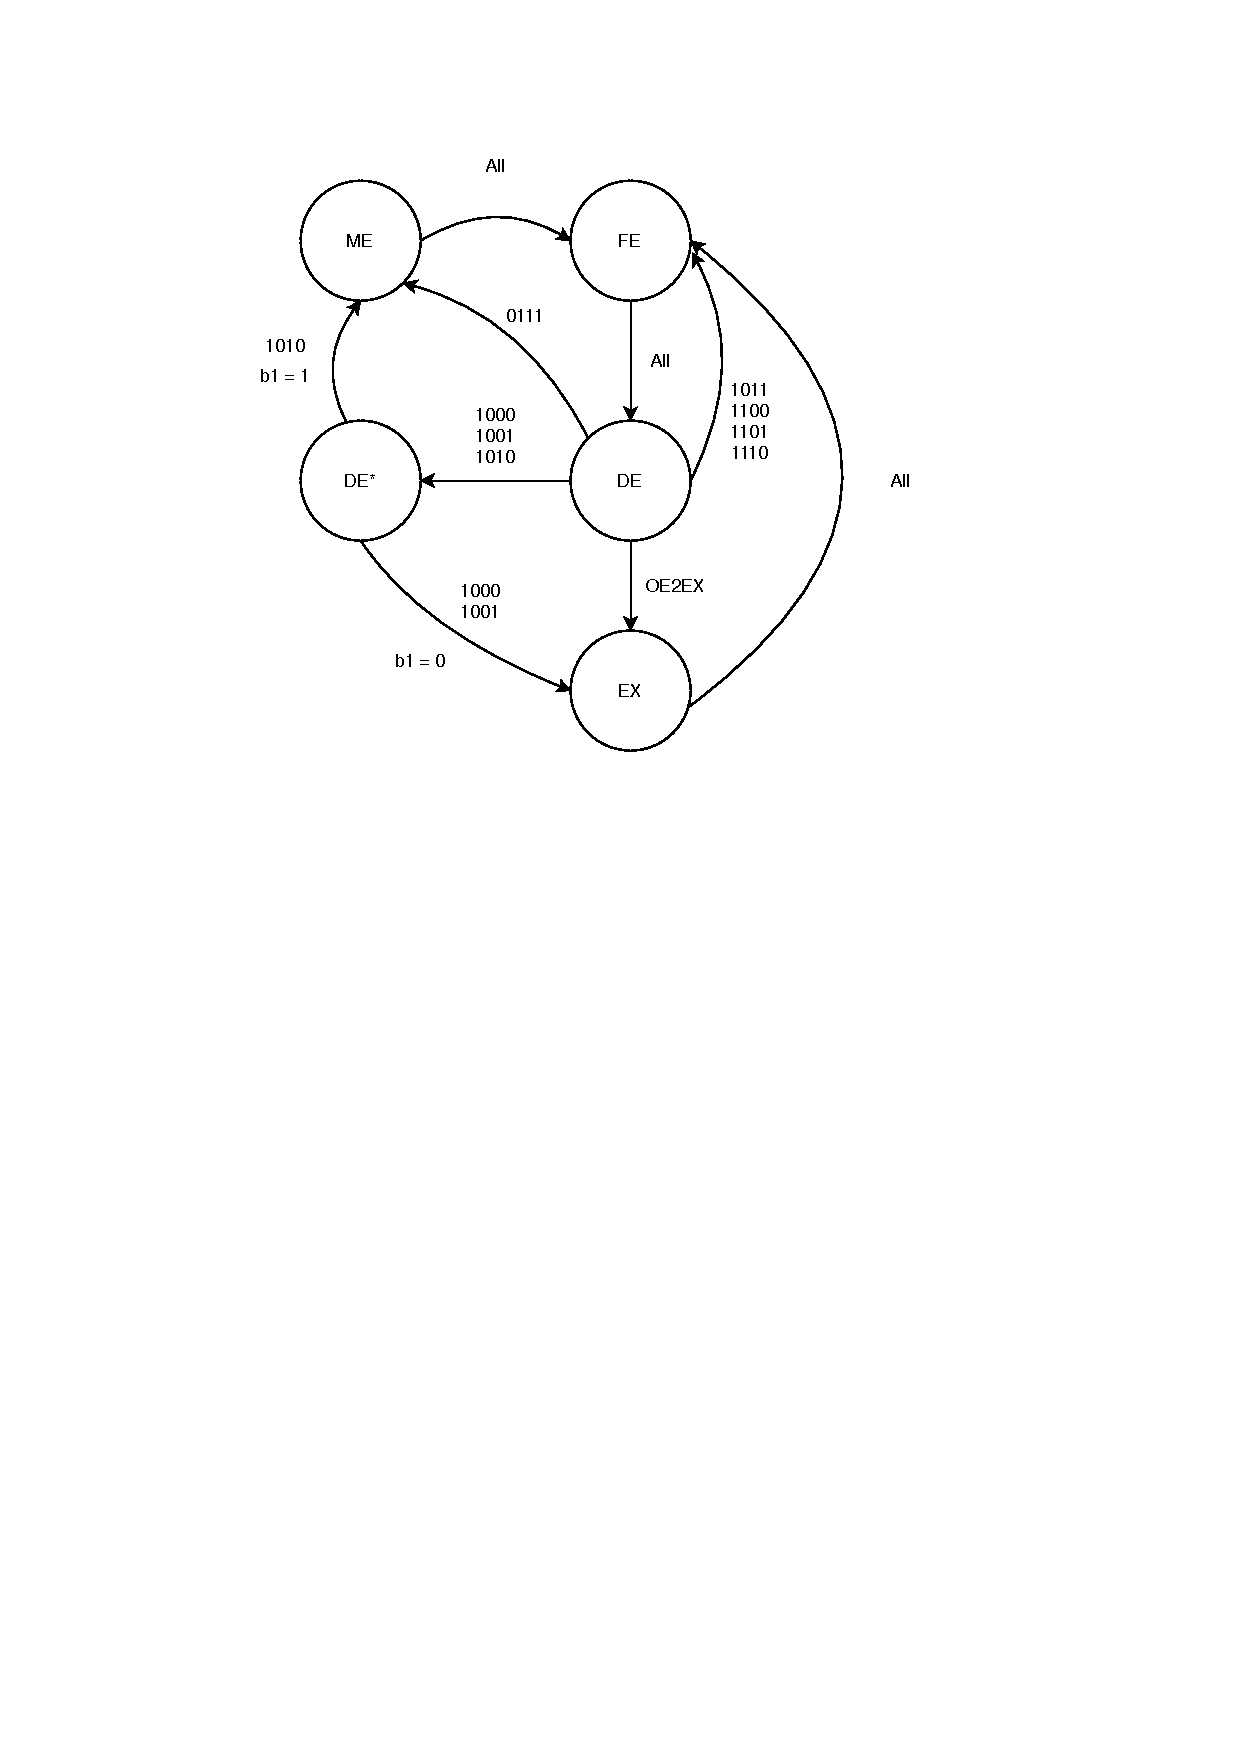
\includegraphics[width=\textwidth]{fsm.pdf}
  \end{figure}


\begin{figure}
    \caption{Waveform showing the correct functionality of the controller.}
    \label{lab3_2:waveform}
    \centering
    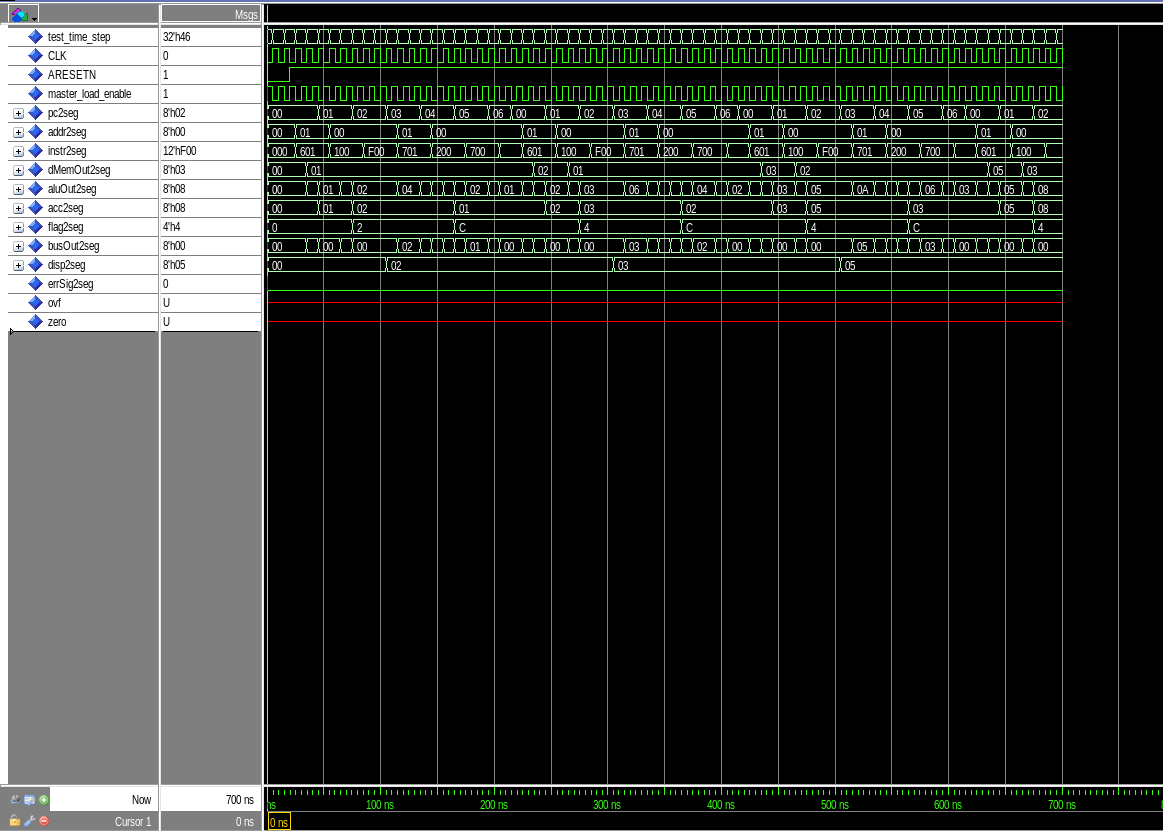
\includegraphics[width=\textwidth]{lab3_waveform.png}
  \end{figure}